% file: main.tex
\documentclass[10pt,oneside]{journal}
\usepackage{mathtools}
\usepackage{fullpage}
\usepackage{listings}
\usepackage{color}
\usepackage{float}
\usepackage{graphicx}
\usepackage[space]{grffile}
\usepackage{endnotes}
\usepackage{natbib}

 
\definecolor{dkgreen}{rgb}{0,0.6,0}
\definecolor{gray}{rgb}{0.5,0.5,0.5}
\definecolor{mauve}{rgb}{0.58,0,0.82}
\definecolor{dkred}{rgb}{0.7,0,0}




\lstset{ %
  language=Python,                % the language of the code
  basicstyle=\small,              % the size of the fonts that are used for the code
  numbers=left,                   % where to put the line-numbers
  numberstyle=\small\color{gray},  % the style that is used for the line-numbers
  stepnumber=1,                   % the step between two line-numbers. If it's 1, each line 
                                  % will be numbered
  numbersep=5pt,                  % how far the line-numbers are from the code
  backgroundcolor=\color{white},      % choose the background color. You must add \usepackage{color}
  showspaces=false,               % show spaces adding particular underscores
  showstringspaces=false,         % underline spaces within strings
  showtabs=false,                 % show tabs within strings adding particular underscores
  frame=single,                   % adds a frame around the code
  rulecolor=\color{black},        % if not set, the frame-color may be changed on line-breaks within not-black text (e.g. commens (green here))
  tabsize=4,                      % sets default tabsize to 2 spaces
  captionpos=b,                   % sets the caption-position to bottom
  breaklines=true,                % sets automatic line breaking
  breakatwhitespace=false,        % sets if automatic breaks should only happen at whitespace
  title=\lstname,                   % show the filename of files included with \lstinputlisting;
                                  % also try caption instead of title
  keywordstyle=\color{blue},          % keyword style
  commentstyle=\color{dkgreen},       % comment style
  stringstyle=\color{mauve},         % string literal style
  escapeinside={\%*}{*)},            % if you want to add a comment within your code
  morekeywords={class,private,procedure,device},               % if you want to add more keywords to the set
  emphstyle=\color{dkred},
  emph={MPI_BCAST,MPI_INTEGER,MPI_COMM_WORLD,ierror,MPI_RECV,MPI_SEND,MPI_DOUBLE_PRECISION,MPI_SCATTER,MPI_GATHER,MPI_INIT,MPI_COMM_SIZE,MPI_COMM_RANK,MPI_WTIME,MPI_BARRIER}
}


\begin{document}
%!TEX root = ../main.tex
% file: title.tex
\begin{center}
\textsc{\Large MCS507 Project Three:\\}
\textsc{Applications of Bayesian Classifiers}
\end{center}
\begin{minipage}{0.6\textwidth}
\begin{flushleft}
	Prepared By: Adam McElhinney
\end{flushleft}
\end{minipage}
\begin{minipage}{0.39\textwidth}
\begin{flushright}
	November 24, 2012
\end{flushright}
\end{minipage}\\[0.01in]
\hrule
%!TEX root = ../main.tex
% file: assignment2.tex


\graphicspath{{C:/Documents and Settings/amcelhinney/My Documents/GitHub/MCS507HW/MCS 507 Homework 4/MCS507--Project-3/tex/include/}}

\section{Assignment One: Overview and Illustrative Example} % (fold)
\label{sec: Main Problem}
Our first objective is to identify the main problem this technique aims to solve. We then provide an overview of the techniques and their implementation. We conclude with an illustrative example that displays the utility of this software.

\subsection{Main Problem this Technique Aims to Solve} % (fold)
\label{sub:methoda}
Bayesian Classifiers broadly refers to a class of tools that rely on Bayes rule to classify objects into various categories. Classification problems are found in nearly every aspect of academic and industrial researching. In particular, Bayesian techniques have proven to be extremely versatile. They have many broad applications in industry and academia. Applications of Bayesian classifiers are found in:

\begin{enumerate}
\item Spam detection
\item Speech Recognition (Merhav)
\item Diagnosis of Dental Pain (Chattopadhyay 2010)
\item Plant Identification
\end{enumerate}

% subsection Main Problem this Software Aims to Solve (end)

\subsection{Overview of the Theory} % (fold)

As stated, Bayesian Classifiers rely on  Bayes theorem, which states for two events \emph{A} and \emph{B}:

\begin{equation}
P(A|B)=\frac{P(B|A)*P(A)}{P(B)}
\end{equation}

\begin{flushleft}We can extend this theorem to any partition of the event space as:
\end{flushleft}

\begin{equation}
P(A_{i}|B)=\frac{P(B|A_{i})*P(A_{i})}{\sum_{j}P(B|A_{j})*P(A_{j})}
\end{equation}

\begin{flushleft}Based on this simple rule, we can address problems of classification by taking a group of observations whose features are known. Then upon finding a suitable probability distribution, we can use Bayes Theorem to calculate the probability that another observation belongs to a certain class, conditional on its features (StatSoft, 2012). 
\end{flushleft}

% subsection Overview of the Theory (end)

\subsection{Illustrative Example} % (fold)

\begin{flushleft}We can illustrate this concept with an example. Suppose that all football teams are either winners or losers. Further, supposed that there are only two football teams on tv that day: the Chicago Bears and the Green Bay Packers. Since the Chicago Bears are such a superior team, they are winners 80\% of the time and therefore losers 20\% of the time. Whereas the Green Bay packers, being inferior in every way, are winners a mere 10\% of the time and therefore losers 90\% of the time. Now suppose upon turning on ESPN to catch the game scores, you hear them refer to a winning team, but cannot make out the name of the team. You would like to know which team they were discussing, but you know that they were either discussing the Chicago Bears or the Green Bay Packers with equal chance. Thus, we can use Bayes Theorem to represent this problem as:
\end{flushleft}

\begin{equation}
P(Bears|Winner)=\frac{P(Winner|Bears)*P(Bears)}{P(Winner)}
\end{equation}

\begin{equation}
P(Winner)=P(Winner|Bears)*P(Bears)+P(Winner|Packers)*P(Packers)
\end{equation}

\begin{flushleft}Using the known values, \begin{math}P(Winner|Bears)=.9\end{math} and \begin{math}P(Bears)=.5\end{math}, we can compute that \begin{math}P(Winner)=.8*.5+.1*.5=.45\end{math}. Finally, this implies
\end{flushleft}
\begin{equation}
P(Bears|Winner)=\frac{.8*.5}{.45}=89\%
\end{equation}
We can thus conclude with nearly 89\% certainty that they were discussing the Chicago Bears and not the Green Bay Packers.


% subsection Illustrative Example (end)

\subsection{Overview of the Methodology} % (fold)

\begin{flushleft}
Now that we have an understanding of Bayes Theorem, we can further discuss the implementation of it for purposes of a Bayesian Classifier. As previously stated, a Bayesian Classifier builds off Bayes theorem to predict membership to a class. If the classifier uses strict assumptions about the independence of the variables, it is referred to as a Niave Bayes Classifier (How to Build a Naive Bayes Classifier, 2012). 
\end{flushleft}
These classifiers are typically implemented using k-fold cross validation. k-fold cross validation is a commonly used machine learning technique where the data is divided into roughly k equal parts (k being specified by the user at the outset). The model is then fit using the observations in k-1 parts. Then the model is then used to score the k-th part. The accuracy of the model is then computed based on its predictive power for this k-th part. This process is repeated k-times, using a different partition each time. The selection of the value k is somewhat arbitrary, but for large data sets, k=10 is generally accepted as a reasonable choice. 

\begin{figure}[H]
    \centering
       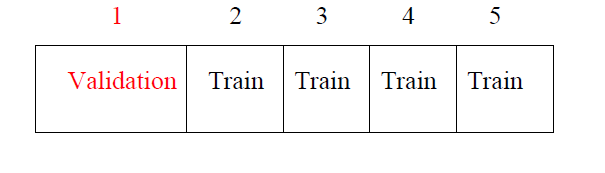
\includegraphics[width=4.5 in]{k-fold_cv.png}
    \caption{Example of k-fold cross-validation, k=5. (Hastie \& Tibshirani 2009)}
    \label{Example Data}
\end{figure}

% subsection Overview of the Methodology (end)

% section Assignment One: Overview and Illustrative Example (end)

%!TEX root = ../main.tex
% file: assignment2.tex


\graphicspath{{C:/Documents and Settings/amcelhinney/My Documents/GitHub/MCS507HW/MCS 507 Homework 4/MCS507--Project-3/tex/include/}}

\section{Assignment Two: Using the Software from Python and A More Substantial Example} % (fold)
\label{sec: Main Problem}
Although our previous example illustrates usage of Bayes Theorem, it is extremely simple and not practical beyond a limited number of specialized cases. Thus, we will now extend this technique to a problem of classification in 2-dimensional space. 

\subsection{Utilizing Bayesian Classifiers in Python} % (fold)

\begin{flushleft}Bayesian Classifiers may be used in Python via the $Orange$ module, which is a module focused on data mining and machine learning. It is also available as a standalone software program complete with a GUI. The $Orange$ module and software is developed by the Bioinformatics Laboratory at the Faculty of Computer and Information Science in the University of Ljubljana, Slovenia (Orange Documentation, 10/20/2012). In addition to the implementation of the Earth software, the $Orange$ module features implementations of the majority of cutting-edge machine learning and data mining techniques, including techniques from the following categories:
\end{flushleft}

\begin{enumerate}
\item Summary Statistics
\item Classification
\item Regression
\item Ensemble Algorithms
\item Clustering
\item Network Analysis
\end{enumerate}

\begin{flushleft}Although the module is written in Python, many of the computations are implemented in C++. This significantly improves the computational speed, while providing the benefits and ease of use of Python.
\end{flushleft}

\subsection{Overview of Example} % (fold)
\begin{flushleft}We know consider the application of Bayesian Classifiers to a simple problem; determining whether an object is likely to be blue, green, or yellow based upon its position (Note that the shapes of the objects were added to provide additional visual distinction and do not represent another dimension of the data). The dots were created manually using the Orange module's data painting feature. The groups were specifically chose such that they have unequal size and that there exists substantial overlap between the groups. 
\end{flushleft}

\begin{table}[H]
\caption{Overview of the Data Set}
\centering
\begin{tabular}{c c}
\hline\hline
Category & Count \\
\hline
Blue & 900 \\
Green & 630 \\
Yellow & 760 \\
\hline
\end{tabular}
\label{table:nonlin} 
\end{table}


\begin{flushleft}We begin our implementation by writing functions to split the data into seperate lists for each class. This will be used later for graphing and scoring purposes. 
\end{flushleft}
\begin{lstlisting}[caption={Partition the Data},label=2nd,firstnumber=16]
########################
# Functions to split the data
########################


def unique(data, class_col):
    """
    Creates a list of unique observations from data
    class_col=the column number containing the group
    """
    groups=[]
    for i in range(len(data)):
        # Check to see if this group has been added to groups
        if data[i][class_col] not in groups:
            groups.append(data[i][class_col])
    return groups


# Split the data into unique groups
def unique_split(data,class_col):
    # Get the list of unique groups
    r=unique(data,class_col)
    p=[]
    for q in range(len(r)):
        p.append([])
    for i in range(len(data)):
        #print i
        for j in range(len(r)):
            #print j
            if data[i][class_col]==r[j]:
                p[j].append(data[i])

    return p
\end{lstlisting}

\begin{flushleft}Next, we import the data using the $C4.5$ data format. This format is common in machine learning as it provides definitions of the variables, as well as explicit type declarations that are understood by the majority of machine learning software tools.  We then split the data into the respective groups.
\end{flushleft}

\begin{lstlisting}[caption={Import the Data and Split},label=2nd,firstnumber=51]
data = orange.ExampleTable("3_groups")
print data.domain.attributes
print data[:4]

# Get a small amount of data
index=Orange.data.sample.SubsetIndices2(p0=0.10)
ind=index(data)
#data_test=data.select(ind,0)
data_test=data


########################
# Split the data
########################

X, Y = data_test.to_numpy("A/C")
data_2=[]
for i in range(len(Y)):
    data_2.append([X[i][0],X[i][1],Y[i]])
p=unique_split(data_2,2)

# Group 1
X11=[p[0][i][0] for i in range(len(p[0]))]
X12=[p[0][i][1] for i in range(len(p[0]))]

# Group 2
X21=[p[1][i][0] for i in range(len(p[1]))]
X22=[p[1][i][1] for i in range(len(p[1]))]

# Group 3
X31=[p[2][i][0] for i in range(len(p[2]))]
X32=[p[2][i][1] for i in range(len(p[2]))]

# Obtain the counts
len(X11);len(X21);len(X31)

\end{lstlisting}

\begin{flushleft}Next, we prepare the data into the form required by $Matplotlib$ and plot the data.
\end{flushleft}

\begin{lstlisting}[caption={Prepare the Data for Plotting; Plot the Data},label=2nd,firstnumber=87]
########################
# Plot the data
########################


import matplotlib.pyplot as plt
import matplotlib
fig = plt.figure()
ax1 = fig.add_subplot(111)

ax1.scatter(X11, X12, s=10, c='b', marker="+")
ax1.scatter(X21, X22, s=10, c='c', marker="o")
ax1.scatter(X31, X32, s=10, c='y', marker="x")
plt.title('Plot of Three Classes of Data')
plt.show()

\end{lstlisting}

\begin{figure}[H]
    \centering
       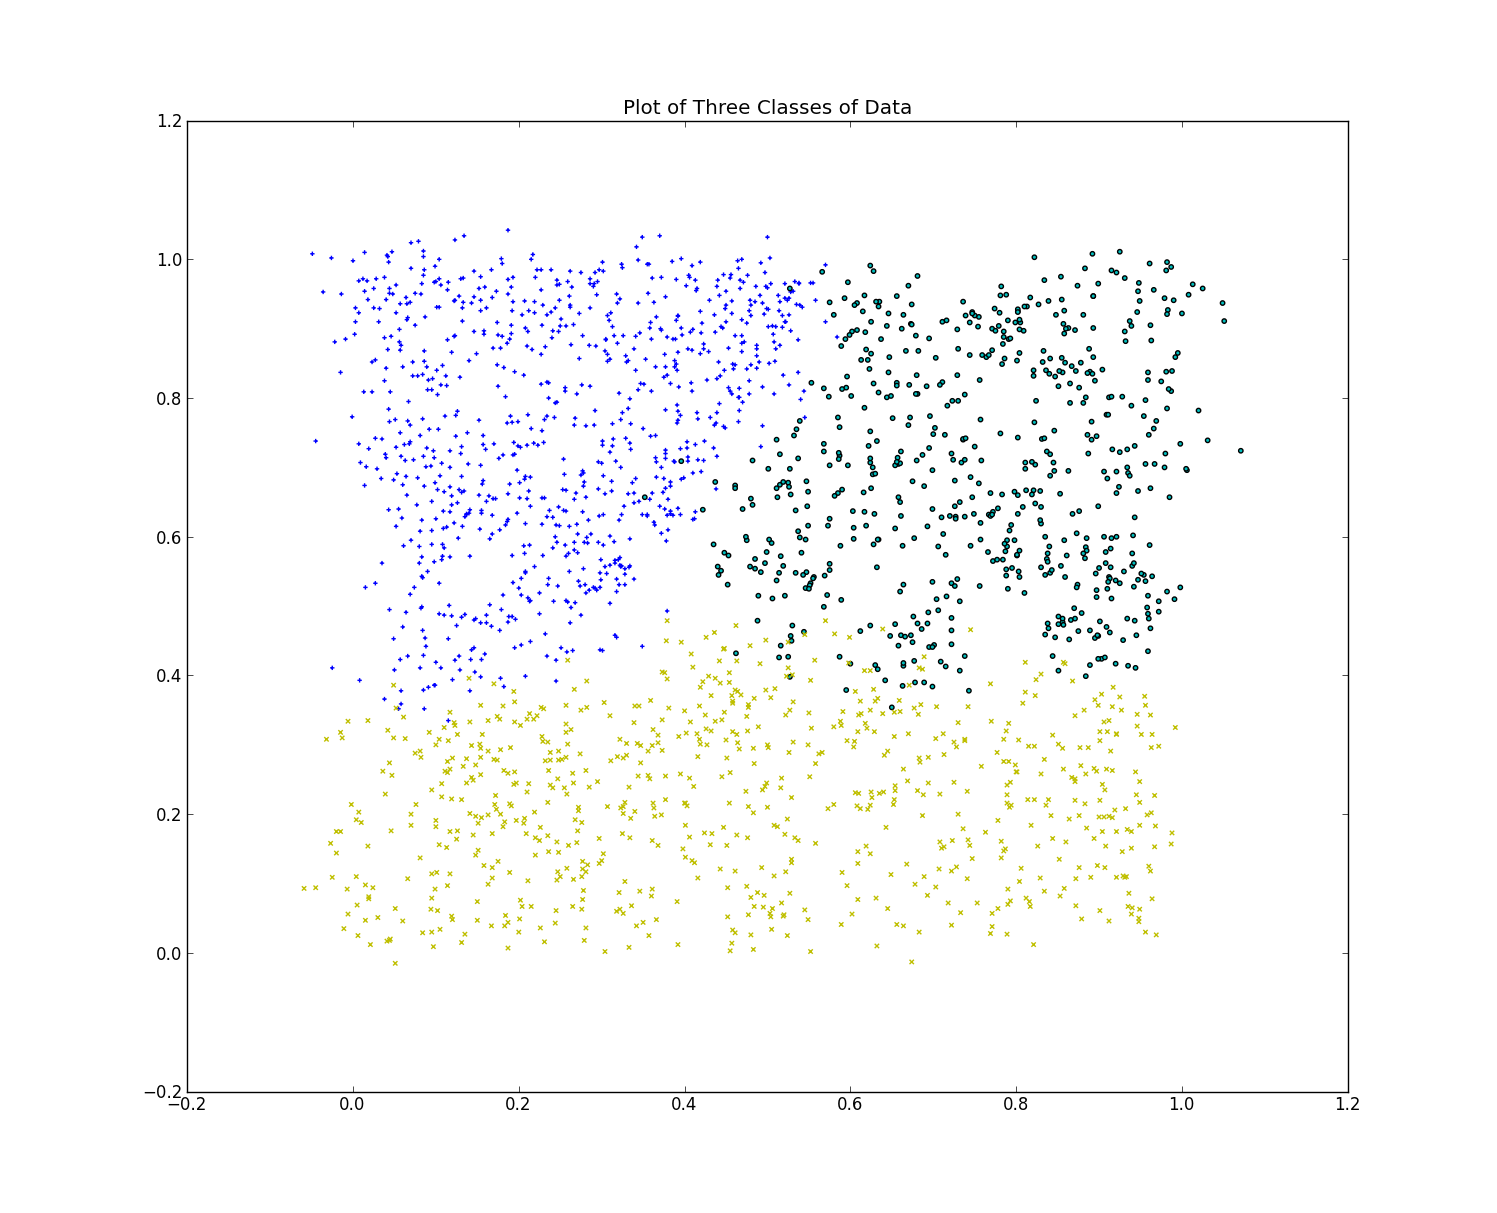
\includegraphics[width=6.5 in]{3_groups.png}
    \caption{Classification of 3 colors in 2-dimensional space}
    \label{Example Data}
\end{figure}


\begin{flushleft}Using the Bayesian methods outlined in the first section, a Naive Bayes Classifier was trained and validated using k-fold cross validation.
\end{flushleft}

\begin{lstlisting}[caption={Construct the Classifier},label=2nd,firstnumber=103]
########################
# Build Classifier
########################

import orange, orngTest, orngStat, orngTree   
classifier = orange.BayesLearner(data)
bayes = orange.BayesLearner()
bayes.name = "bayes"
learners = [bayes]

results = orngTest.crossValidation(learners, data_test, folds=10)
\end{lstlisting}

\begin{flushleft}Once the classifier is constructed, we wish to compute the misclassified operations. The package $Orange$ provides a convienent way of doing this, however it cannot interface directly with $Matplotlib$. Thus, the data was converted to $NumPy$ arrays.
\end{flushleft}

\begin{lstlisting}[caption={Compute the Misclassified Observations},label=2nd,firstnumber=115]
########################
# Compute the misclassified observations
########################

X, Y = data_test.to_numpy("A/C")
data_scored=[]
for i in range(len(results.results)):
    if results.results[i].classes[0]==results.results[i].actual_class:
        data_scored.append(1)
    else:
        data_scored.append(0)

import matplotlib.pyplot as plt
import matplotlib

X1w=[];X2w=[]
for i in range(len(X)):
    if data_scored[i]==0:
        X1w.append(X[i][0])
        X2w.append(X[i][1])
\end{lstlisting}

\begin{flushleft}We now overlay the misclassified observations onto plots of the data points to give a visual approximation of how successful is our classifier.
\end{flushleft}

\begin{lstlisting}[caption={Compute the Misclassified Observations},label=2nd,firstnumber=123]
########################
# Plot the misclassified data
########################
fig = plt.figure()
ax1 = fig.add_subplot(111)

ax1.scatter(X11, X12, s=10, c='b', marker="+")
ax1.scatter(X21, X22, s=10, c='c', marker="o")
ax1.scatter(X31, X32, s=10, c='y', marker="x")
ax1.scatter(X1w, X2w, s=10, c='m', marker="^")
plt.title('Plot of Three Classes of Data, Showing the Misclassified Elements')
plt.show()
\end{lstlisting}

\begin{figure}[H]
    \centering
       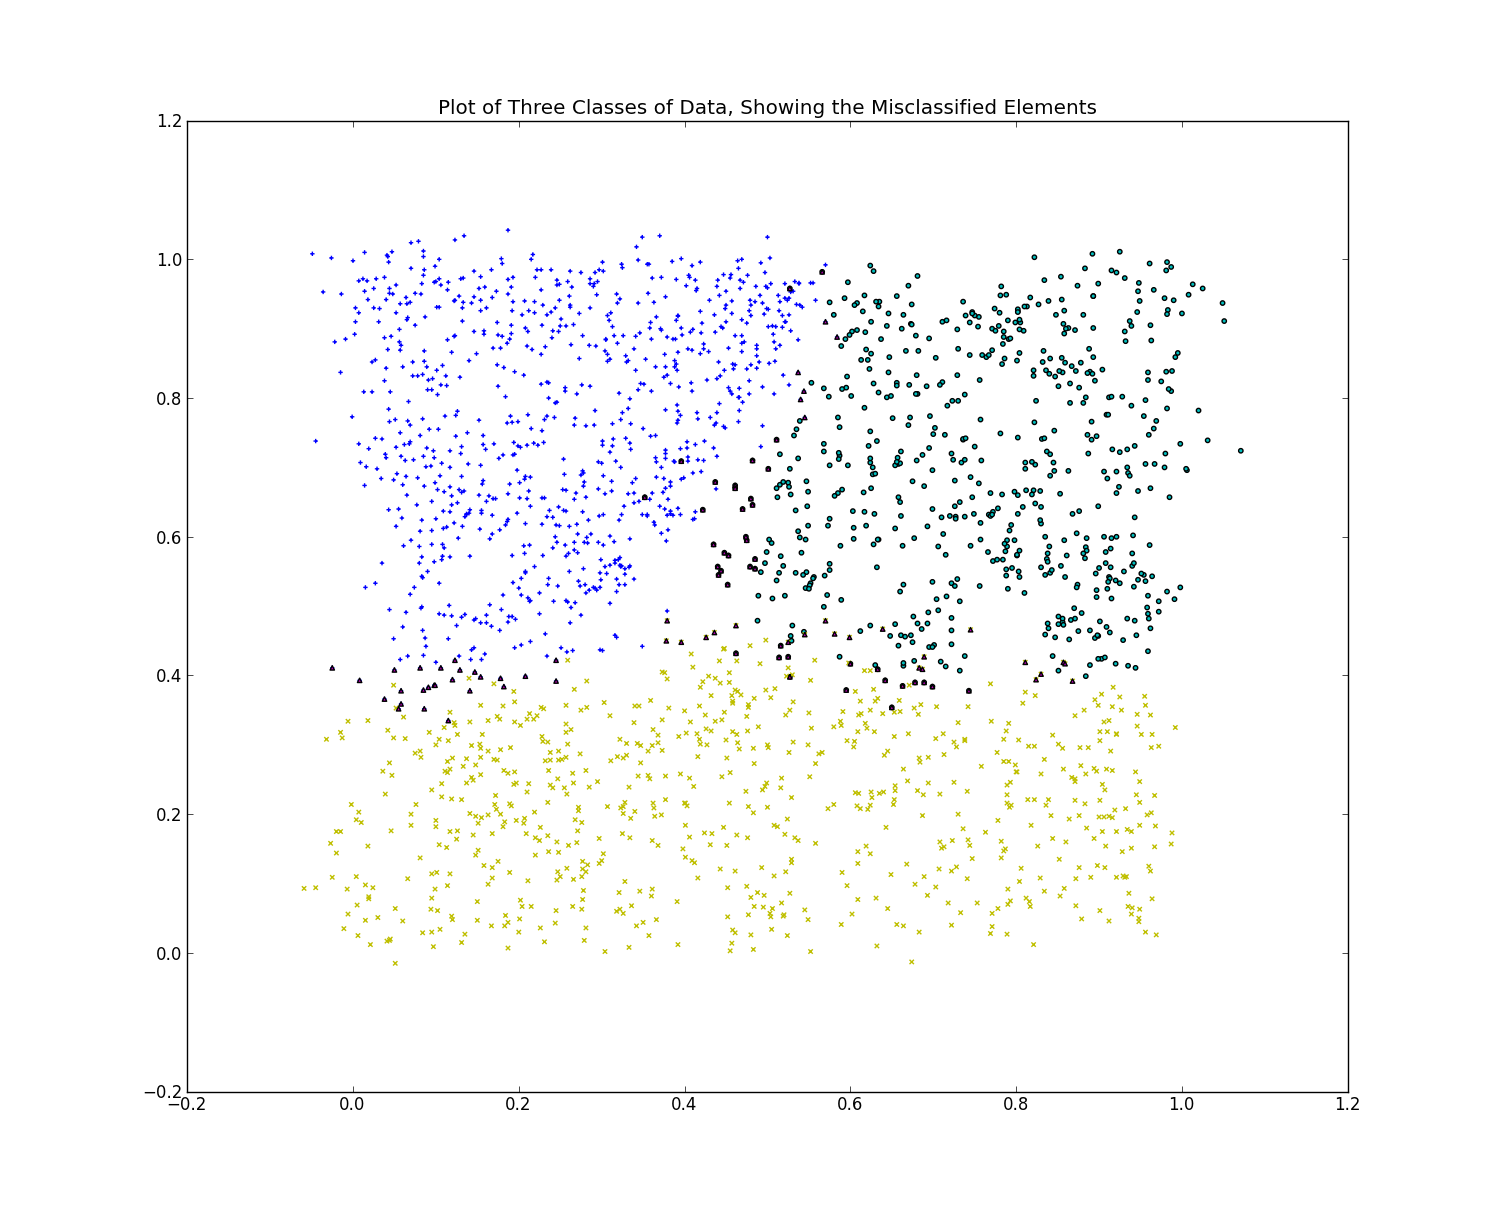
\includegraphics[width=6.5 in]{3_groups_mis.png}
    \caption{Classification of 3 colors in 2-dimensional space; Misclassifications displayed}
    \label{Example Data}
\end{figure}

\begin{flushleft}As the above figure shows, our classifier is quite successful. We see a small number of misclassified observations (represented as dark triangles) that predictably lie in the boundaries between the three groups. However, in addition to a visual representation of the accuracy of the classifier, the $Orange$ package provides us with a full range of summary statistics to assess the model performance. 
\end{flushleft}
\begin{lstlisting}[caption={Compute the Misclassified Observations},label=2nd,firstnumber=151]
# output the results
print "Learner CA IS Brier AUC"
for i in range(len(learners)):
    print "%-8s %5.3f %5.3f %5.3f %5.3f" % (learners[i].name, \
    orngStat.CA(results)[i], orngStat.IS(results)[i], orngStat.BrierScore(results)[i], orngStat.AUC(results)[i])
\end{lstlisting}

\begin{table}[H]
\caption{Model Performance Statistics}
\centering
\begin{tabular}{c c}
\hline\hline
Statistics & Value\\
\hline
Classification Accuracy & 96\% \\
Information Score & 1.301\\
Brier Score & .093\\
Area Under ROC &.998\\
\hline
\end{tabular}
\label{table:nonlin} 
\end{table}

\begin{flushleft}The exact definitions of all of these metrics is beyond the scope of this paper. However, one metric to call out is the Classification Accuracy. This is simply the percentage of observations that are classified correctly. The value of 96\% represents an excellent classifier. This intuitively matches our observations based on the graph of misclassifications.
\end{flushleft}

% subsection Overview of Example (end)




% section Assignment One: Overview and Illustrative Example (end)

%!TEX root = ../main.tex
% file: assignment2.tex


%\graphicspath{{C:/Documents and Settings/amcelhinney/My Documents/GitHub/MCS507_Final_Project/tex/include}}
\graphicspath{{C:/Documents and Settings/amcelhinney/My Documents/GitHub/MCS507--Project-3/tex/include/}}

\section{Assignment Three: A More Substantial Example} % (fold)
\subsection{Overview of Example} % (fold)
\begin{flushleft}We know consider the application of Bayesian Classifiers to a simple problem; determining whether an object is likely to be blue, green, or yellow based upon its position (Note that the shapes of the objects were added to provide additional visual distinction and do not represent another dimension of the data). The dots were created manually using the $Orange$ module's data painting feature. The groups were specifically chose such that they have unequal size and that there exists substantial overlap between the groups. 
\end{flushleft}

\begin{table}[H]
\caption{Overview of the Data Set}
\centering
\begin{tabular}{c c}
\hline\hline
Category & Count \\
\hline
Blue & 900 \\
Green & 630 \\
Yellow & 760 \\
\hline
\end{tabular}
\label{table:nonlin} 
\end{table}


\begin{flushleft}We begin our implementation by writing functions to split the data into separate lists for each class. This will be used later for graphing and scoring purposes. 
\end{flushleft}
\begin{lstlisting}[caption={Partition the Data},label=2nd,firstnumber=16]
########################
# Functions to split the data
########################


def unique(data, class_col):
    """
    Creates a list of unique observations from data
    class_col=the column number containing the group
    """
    groups=[]
    for i in range(len(data)):
        # Check to see if this group has been added to groups
        if data[i][class_col] not in groups:
            groups.append(data[i][class_col])
    return groups


# Split the data into unique groups
def unique_split(data,class_col):
    # Get the list of unique groups
    r=unique(data,class_col)
    p=[]
    for q in range(len(r)):
        p.append([])
    for i in range(len(data)):
        #print i
        for j in range(len(r)):
            #print j
            if data[i][class_col]==r[j]:
                p[j].append(data[i])

    return p
\end{lstlisting}

\begin{flushleft}Next, we import the data using the $C4.5$ data format. This format is common in machine learning as it provides definitions of the variables, as well as explicit type declarations that are understood by the majority of machine learning software tools.  We then split the data into the respective groups.
\end{flushleft}

\begin{lstlisting}[caption={Import the Data and Split},label=2nd,firstnumber=51]
data = orange.ExampleTable("3_groups")
print data.domain.attributes
print data[:4]

# Get a small amount of data
index=Orange.data.sample.SubsetIndices2(p0=0.10)
ind=index(data)
#data_test=data.select(ind,0)
data_test=data


########################
# Split the data
########################

X, Y = data_test.to_numpy("A/C")
data_2=[]
for i in range(len(Y)):
    data_2.append([X[i][0],X[i][1],Y[i]])
p=unique_split(data_2,2)

# Group 1
X11=[p[0][i][0] for i in range(len(p[0]))]
X12=[p[0][i][1] for i in range(len(p[0]))]

# Group 2
X21=[p[1][i][0] for i in range(len(p[1]))]
X22=[p[1][i][1] for i in range(len(p[1]))]

# Group 3
X31=[p[2][i][0] for i in range(len(p[2]))]
X32=[p[2][i][1] for i in range(len(p[2]))]

# Obtain the counts
len(X11);len(X21);len(X31)

\end{lstlisting}

\begin{flushleft}Next, we prepare the data into the form required by $Matplotlib$ and plot the data.
\end{flushleft}

\begin{lstlisting}[caption={Prepare the Data for Plotting; Plot the Data},label=2nd,firstnumber=87]
########################
# Plot the data
########################


import matplotlib.pyplot as plt
import matplotlib
fig = plt.figure()
ax1 = fig.add_subplot(111)

ax1.scatter(X11, X12, s=10, c='b', marker="+")
ax1.scatter(X21, X22, s=10, c='c', marker="o")
ax1.scatter(X31, X32, s=10, c='y', marker="x")
plt.title('Plot of Three Classes of Data')
plt.show()

\end{lstlisting}

\begin{figure}[H]
    \centering
       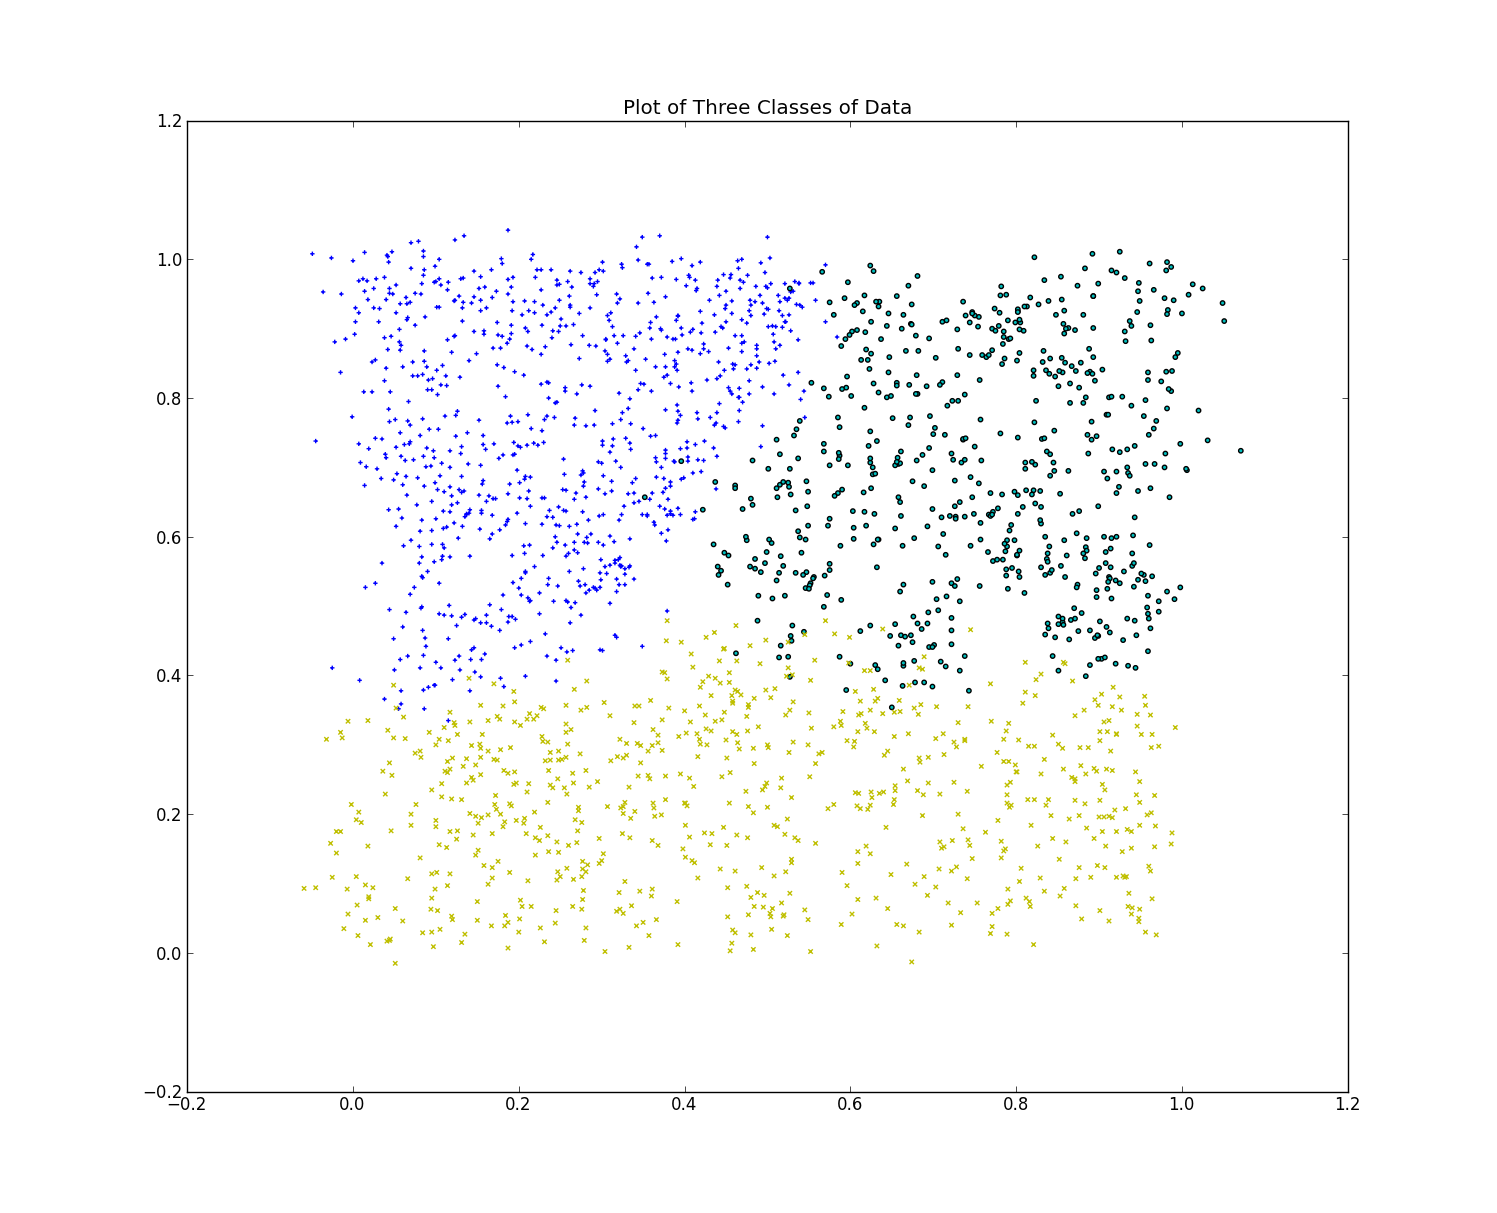
\includegraphics[width=6.5 in]{3_groups.png}
    \caption{Classification of 3 colors in 2-dimensional space}
    \label{Example Data}
\end{figure}


\begin{flushleft}Using the Bayesian methods outlined in the first section, a Naive Bayes Classifier was trained and validated using k-fold cross validation.
\end{flushleft}

\begin{lstlisting}[caption={Construct the Classifier},label=2nd,firstnumber=103]
########################
# Build Classifier
########################

import orange, orngTest, orngStat, orngTree   
classifier = orange.BayesLearner(data)
bayes = orange.BayesLearner()
bayes.name = "bayes"
learners = [bayes]

results = orngTest.crossValidation(learners, data_test, folds=10)
\end{lstlisting}

\begin{flushleft}Once the classifier is constructed, we wish to compute the misclassified operations. The package $Orange$ provides a convenient way of doing this, however it cannot interface directly with $Matplotlib$. Thus, the data was converted to $NumPy$ arrays.
\end{flushleft}

\begin{lstlisting}[caption={Compute the Misclassified Observations},label=2nd,firstnumber=115]
########################
# Compute the misclassified observations
########################

X, Y = data_test.to_numpy("A/C")
data_scored=[]
for i in range(len(results.results)):
    if results.results[i].classes[0]==results.results[i].actual_class:
        data_scored.append(1)
    else:
        data_scored.append(0)

import matplotlib.pyplot as plt
import matplotlib

X1w=[];X2w=[]
for i in range(len(X)):
    if data_scored[i]==0:
        X1w.append(X[i][0])
        X2w.append(X[i][1])
\end{lstlisting}

\begin{flushleft}We now overlay the misclassified observations onto plots of the data points to give a visual approximation of how successful is our classifier.
\end{flushleft}

\begin{lstlisting}[caption={Compute the Misclassified Observations},label=2nd,firstnumber=123]
########################
# Plot the misclassified data
########################
fig = plt.figure()
ax1 = fig.add_subplot(111)

ax1.scatter(X11, X12, s=10, c='b', marker="+")
ax1.scatter(X21, X22, s=10, c='c', marker="o")
ax1.scatter(X31, X32, s=10, c='y', marker="x")
ax1.scatter(X1w, X2w, s=10, c='m', marker="^")
plt.title('Plot of Three Classes of Data, Showing the Misclassified Elements')
plt.show()
\end{lstlisting}

\begin{figure}[H]
    \centering
       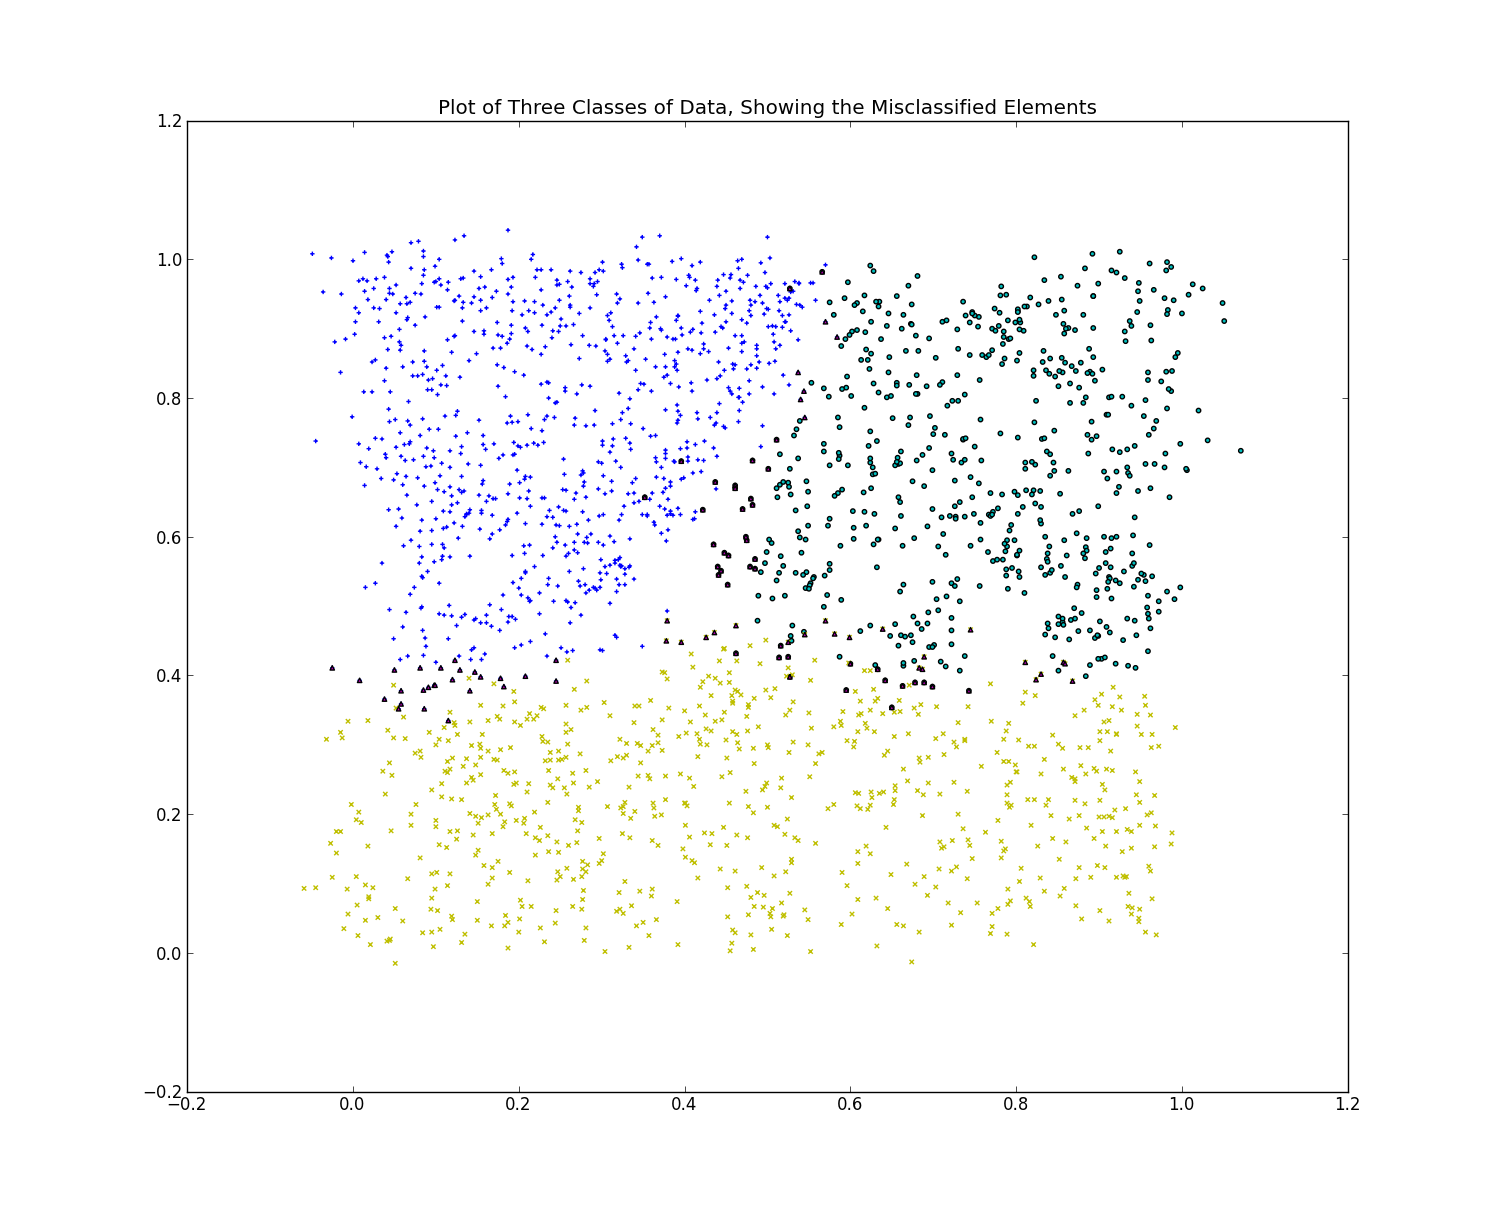
\includegraphics[width=6.5 in]{3_groups_mis.png}
    \caption{Classification of 3 colors in 2-dimensional space; Misclassifications displayed}
    \label{Example Data}
\end{figure}

\begin{flushleft}As the above figure shows, our classifier is quite successful. We see a small number of misclassified observations (represented as dark triangles) that predictably lie in the boundaries between the three groups. However, in addition to a visual representation of the accuracy of the classifier, the $Orange$ package provides us with a full range of summary statistics to assess the model performance. 
\end{flushleft}
\begin{lstlisting}[caption={Compute the Misclassified Observations},label=2nd,firstnumber=151]
# output the results
print "Learner CA IS Brier AUC"
for i in range(len(learners)):
    print "%-8s %5.3f %5.3f %5.3f %5.3f" % (learners[i].name, \
    orngStat.CA(results)[i], orngStat.IS(results)[i], orngStat.BrierScore(results)[i], orngStat.AUC(results)[i])
\end{lstlisting}

\begin{table}[H]
\caption{Model Performance Statistics}
\centering
\begin{tabular}{c c}
\hline\hline
Statistics & Value\\
\hline
Classification Accuracy & 96\% \\
Information Score & 1.301\\
Brier Score & .093\\
Area Under ROC &.998\\
\hline
\end{tabular}
\label{table:nonlin} 
\end{table}

\begin{flushleft}The exact definitions of all of these metrics is beyond the scope of this paper. However, one metric to call out is the Classification Accuracy. This is simply the percentage of observations that are classified correctly. The value of 96\% represents an excellent classifier. This intuitively matches our observations based on the graph of misclassifications.
\end{flushleft}

% subsection Overview of Example (end)




% section Assignment One: Overview and Illustrative Example (end)

%!TEX root = ../main.tex
% file: assignment2.tex


\graphicspath{{C:/Documents and Settings/amcelhinney/My Documents/GitHub/MCS507ProjectTwo/tex/include/}}

\section{Conclusion} % (fold)
We have shown how the $Orange$ software package implements the Bayesian Classifiers and how it can be very useful for quickly solving real world problems. Some areas of consideration for additional explanation are:
\begin{enumerate}
\item Evaluation on another "real-world" data set
\item High dimensional data (data sets where there are a much larger amount of explanatory variables as compared with the number of observations)
\item Comparison with other classifiers (Support vector machines, Neural Networks, etc)
\end{enumerate}

In summation, Bayesian Classifiers are a versatile tool with applications to real world data sets. 
%!TEX root = ../main.tex
% file: assignment2.tex


\graphicspath{{C:/Documents and Settings/amcelhinney/My Documents/GitHub/MCS507ProjectTwo/tex/include/}}
\newpage

\section{Bibliography} % (fold)

\hspace{5 mm}About. (2012). Orange. Retrieved 10/20/2012 from http://orange.biolab.si/about/\\

Chattopadhyay S, Davis RM, Menezes DD, Singh G, Acharya RU, Tamura T. "Application of Bayesian classifier for the diagnosis of dental pain." J Med Syst. 2012 Jun;36(3):1425-39. Epub 2010 Oct 13. \\

Cross-Validation. (2012). Wikipedia. Retrieved 11/18/2012 from \\
https://en.wikipedia.org/wiki/Cross-validation\_\%28statistics\%29

\hspace{5 mm} Hastie \& Tibshirani."Cross-validation and bootstrap". Retrieved from www-stat.stanford.edu/\~tibs/sta306b/cvwrong.pdf, November 27, 2012.\\

How To Build a Naive Bayes Classifier. Retrieved 11/20/2012 from \\http://bionicspirit.com/blog/2012/02/09/howto-build-naive-bayes-classifier.html/\\

Naive Bayes classifier. (2012). Wikipedia. Retrieved 11/18/2012 from \\
https://en.wikipedia.org/wiki/Naive\_Bayes\_classifier\\

StatSoft Electronic Statistics Textbook. Naive Bayes Classifier. StatSoft. Retrieved 11/15/2012 from 
\\http://www.statsoft.com/textbook/\\


%\bibliography{refs}
%\bibliographystyle{plain}


	

	
	
\end{document}